\documentclass[conference]{IEEEtran}
\IEEEoverridecommandlockouts
% The preceding line is only needed to identify funding in the first footnote. If that is unneeded, please comment it out.
\usepackage{cite}
\usepackage{amsmath,amssymb,amsfonts}
\DeclareUnicodeCharacter{2009}{\,} 
\usepackage{algorithmic}
\usepackage{graphicx}
\usepackage{hyperref}
\usepackage{textcomp}
\usepackage{xcolor}
\def\BibTeX{{\rm B\kern-.05em{\sc i\kern-.025em b}\kern-.08em
    T\kern-.1667em\lower.7ex\hbox{E}\kern-.125emX}}

\makeatletter
\newcommand{\linebreakand}{%
  \end{@IEEEauthorhalign}
  \hfill\mbox{}\par
  \mbox{}\hfill\begin{@IEEEauthorhalign}
}
\makeatother

\begin{document}

\title{Prognosticate Dunes on the surface of Mars using Convolutional Neural Network\\}

\author{\IEEEauthorblockN{1\textsuperscript{st} Anurag Dutta}
\IEEEauthorblockA{\textit{Department of Computer Science} \\
\textit{Government College of Engineering \& Textile Technology}\\
Serampore, Calcutta, India \\
anuragdutta.research@gmail.com}
\and 
\IEEEauthorblockN{2\textsuperscript{nd} A. Ramamoorthy}
\IEEEauthorblockA{\textit{Department of Mathematics} \\
\textit{Velammal Engineering College, Anna University}\\
Chennai, Tamil Nadu, India \\
ramzenithmaths@gmail.com}
\linebreakand
\IEEEauthorblockN{3\textsuperscript{rd} Ritvik Sharma}
\IEEEauthorblockA{\textit{Department of Computer Science} \\
\textit{SRM Institute of Science \& Technology}\\
Delhi - NCR Campus, Uttar Pradesh, India \\
ritvikdevelops@gmail.com}
\and
\IEEEauthorblockN{4\textsuperscript{th} Unnati Sadh}
\IEEEauthorblockA{\textit{Department of Computer Science} \\
\textit{SRM Institute of Science \& Technology}\\
Delhi - NCR Campus, Uttar Pradesh, India \\
unnatisadh819@gmail.com}
\linebreakand
\IEEEauthorblockN{5\textsuperscript{th} John Harshith}
\IEEEauthorblockA{\textit{Department of Computer Science} \\
\textit{Vellore Institute of Technology, Vellore Campus}\\
Vellore, Tamil Nadu, India\\
johnharshith@icloud.com}
}

\maketitle

\begin{abstract}
In the past few years, technological boom have efficiently helped mankind a lot. May it be Artificial Intelligence, or Internet of Things, we humans have been using these newer technologies almost everyday. Amongst all, Artificial Intelligence is a technology stack, or a conception, that have caught great heights. Starting from the innovation of Deep Blue, by IBM to development of self driving cars by Google, AI have it's blanket worn on humans today. In this work, we would make use of Artificial Intelligence, to be specific, Neural Network, to predict vulnerability of dunes on the surface of Mars. Almost all Space Agencies are planing their manned mission to Mars. The perchlorate salt is present in amounts of 0.6\% in Martian soil, that has an alkaline pH of 7.7 and is poisonous to humans. Even if we manage to overcome the alkalinity, the dunes on the surface of Mars, makes it difficult for landing a rover on it's surface. Making use of Convolutional Neural Network, we would train a model that would be efficient enough to predict the dunes on the surface of Mars. If we are able to predict the presence of dunes on a particular strata of the Martian Crust, we would prefer landing the rover on some different patch. This would reduce chances of threats and damage to the rover. Several orbiters are spawned on the Mars. One of the oldest being \textit{Mars Reconnaissance Orbiter}, launched by NASA in 2005. MRO have sent numerous pictures of Mars' Crust. In this work, we would make use of such data to train the Neural Network in epochs. Alongside, we have also made use of the traditional Machine Learning Classifiers to predict the same, which resulted in a big contrast to the accuracy of the prediction made using the 4 - Layer Convolutional Neural Network Model. \\
\end{abstract}
\begin{IEEEkeywords}
Mars Reconnaissance Orbiter, Martian Dunes, Artificial Intelligence, Artificial Neural Network
\end{IEEEkeywords}
\section{Introduction}
Mars, the solar system's [1] second-smallest planet, is located 3 planets away from the sun. It is just larger than Mercury, which is the planet that is the closest to the Sun [2]. The Roman god of war was given the name Mars in English, and the planet is named after him. Mars is a terrestrial planet that has a thin atmosphere even less than 1\% of that of Earth, a crust that is mostly composed of elements comparable to Earth's crust, and a core that is built of iron and nickel. Impact craters, valleys, dunes, and polar ice caps are some of the surface features that can be found on Mars. \textit{Phobos} [3] and \textit{Deimos} [4], its two moons, are both relatively small and have an asymmetrical shape. One of the longest gorges throughout the Solar System as well as the largest volcano in the Solar System, \textit{Olympus Mons} [5], are two of Mars' most remarkable surface features. Olympus Mons is also the planet's tallest known mountain. About 40 percent of the planet's surface is taken up by the Borealis basin throughout the Northern Hemisphere, which could be a significant impact feature. Mars has seasons and days that are similar to those of Earth because of the planets' shared rotation periods and ecliptic plane-inclined tilts of their revolving axes. Because Mars' atmospheric pressure is so low, less than 1\% of that of Earth, therefore liquid water cannot exist on the planet's surface. It appears that water makes up the majority of both of Mars' polar ice caps. Mars was probably wetter and so more conducive to life in the distant past. It is unknown if there has ever been life on Mars. Since \textit{Mariner 4}'s launch in 1965, a number of unmanned spacecraft have investigated Mars. In 1976, the \textit{Viking 1} [6] lander by NASA successfully sent back the first photographic images captured on Mars. Both, China and the United States with \textit{Zhurong} [7] and \textit{Sojourner} [8], respectively have successfully launched rovers on Mars. Future Mars missions are also being planned, including the \textit{NASA-ESA Mars Sample Return} [9] in 2026 as well as the \textit{Rosalind Franklin rover expedition} [10], which was originally scheduled to launch in 2018 but will now most likely launch in 2028. Mars and its reddish hue are visible to the naked eye from Earth. Mars is frequently referred to as the \textit{Red Planet} because of its appearance, which is caused by the abundance of iron oxide on its surface. With an apparent brightness of up to 2.94, comparable to Jupiter's, it is one of the brightest objects in the Earth's night sky, only being surpassed by Venus, the Moon, and the Sun. Since ancient times, Mars has been seen, and throughout the ages, it has been depicted in the arts and culture in ways that reflect humanity's expanding understanding of it. A spacecraft called the \textit{Mars Reconnaissance Orbiter} [11] is intended to investigate the geology and temperature of Mars, offer information about potential landing locations, and transmit the data of surface missions back to Earth. On March 10, 2006, it arrived on Mars after being shot on August 12, 2005. Following five months of aerobraking [12], it attained its penultimate science orbit and started its primary science phase in November 2006. \\

An interplanetary vehicle must slow down when it reaches its destination in order to enter orbit or land. The required velocity variations may be on the scale of kilometres per second to achieve a low, roughly circular trajectory around a planet with significant gravity (as is necessary for many scientific experiments). The rocket equation requires that a significant portion of the mass of the spacecraft be made up of fuel in order to use propulsion. As a result, the science payload is reduced,or a big, expensive rocket is needed. \textit{Aerobraking} can be utilised to lower the amount of fuel needed, provided the destination body has an atmosphere. The spacecraft can enter an extended elliptic orbit by using a relatively short burn. The orbit is then circularised by aerobraking. If the airspace is dense enough, the orbit can be changed with just one pass. Aerobraking, however, often necessitates many orbits deeper in the atmosphere. As a result, frictional heating, erratic turbulence effects, air composition, and temperature are lessened. This kind of aerobraking gives enough time between passes to evaluate the velocity difference and make adjustments for the subsequent pass. For Mars, completing the final orbit could take more than six months and involve numerous laps through the atmosphere. For the spacecraft to raise the periapsis above the atmosphere after the final pass, it needs to be supplied more kinetic energy by rocket engines.
\section{Martian Terrains}
Basaltic rock [13], or material created by molten lava, makes up the surface of Mars. However, scientists discovered higher silicon concentrations in meteorite-extracted material from kilometres below the surface. The bleak, barren wastelands of Mars are dotted with impact craters and ancient volcanoes. The entire area can be covered by a single sandstorm, blocking out sight for a few days at a time. Despite the difficult conditions, researchers know more about the surface of Mars than any other place in the Solar System. It's a small world on Mars. It has a mass of less than one tenth that of the Earth and a radius that is half that of the planet. The surface area of the Red Planet is comparable to 25\% of Earth. Even though it doesn't seem like a big world, it is almost equal to the entire dry land of Earth. The surface is believed to be primarily made of basalt and covered in a thin coating of talcum-like iron oxide dust. Iron oxide is responsible for the planet's distinctive red colour. Volcanoes were able to erupt unchecked for millions of years in the planet's distant history. Mars lacks plate tectonics, therefore a single hotspot might deposit molten rock on the surface for ages. Because there were no tectonic movements, the same surface breach persisted until there was no longer enough pressure to push magma to the surface. This is how \textit{Olympus Mons}, the biggest peak in the Solar System, formed. Three times as tall as Mount Everest, it. The deepest valley in the Solar System may possibly be partially explained by these rogue volcanic events. \textit{Valles Marineris} [14], which is also on Mars, is believed to have formed as a result of the material collapsing between two hotspots. Impact craters are scattered across the Martian surface. Due to the lack of environmental pressures that would degrade them, the majority of these craters have remained in tact. The erosion-causing factors present on Earth, such as wind, storm, and plate tectonics, do not exist on the planet. Because it has a thinner atmosphere than Earth, smaller meteorites can strike the planet. The surface of Mars is thought to have changed significantly over the course of billions of years. Numerous minerals and erosional patterns on the planet imply the presence of liquid water in the past, according to data collected by rovers and orbiters. It's probable that the area was originally dominated by long rivers and little oceans. Below the surface, the final traces of the water are frozen into water ice. Some of the ice will be examined by scientists in an effort to unearth hidden Martian treasures. Figure 1 shows a surficial image of Mars' Surface. 
\begin{figure}[htbp]
\label{fig1}
\centerline{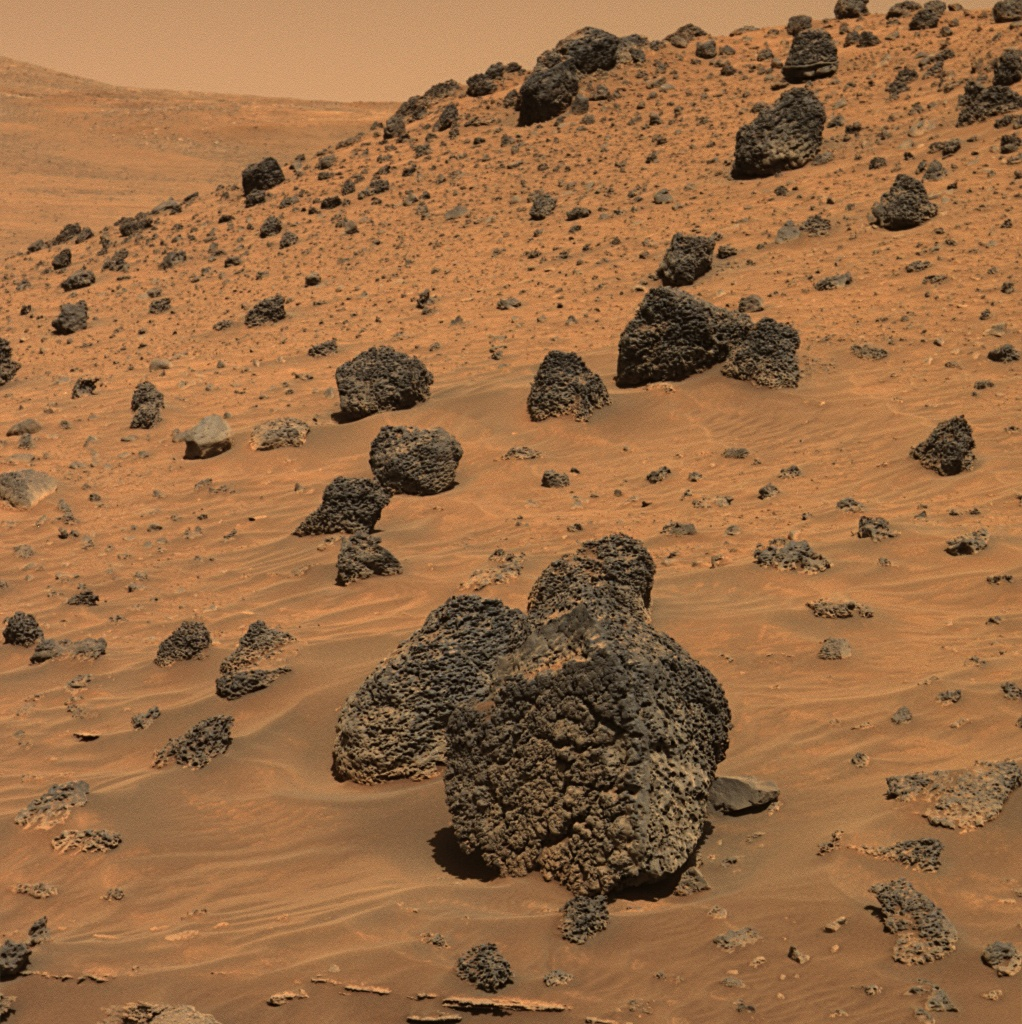
\includegraphics[width = \linewidth]{1}}
\caption{A picture of the rocky and dusty terrain of Mars taken by a Mars rover.}
\end{figure}
\section{Convolutional Neural Network}
A CNN, or \textit{Convolutional Neural Network} [15], is a type of deep learning neural network designed for processing organised arrays of input, such as photos. \textit{Convolutional Neural Network}, the state-of-the-art for many visual applications including image categorization, are frequently used in computer vision. \textit{Convolutional Neural Network} are capable of quickly recognizing trends like bars, gradients, curves, or even eyes and faces in the input image. This characteristic makes \textit{Convolutional Neural Network} very useful for Computer Vision. Unlike earlier Computer Vision [16] techniques, \textit{Convolutional Neural Network} can start working on a raw image right away and do not need any preparation. \textit{Convolutional Neural Network} are feed-forward neural networks with up to 20 or 30 layers. \textit{Convolutional Neural Network} strength comes from a special type of layer called the Convolutional layer. In CNNs, many convolution layer are stacked on top of another, and each level is able to recognize increasingly intricate structures. Handwritten digits can be recognised with three or four Convolutional layers, while human faces can be distinguished with 25 layers. \\

The architecture of a Convolutional Network is composed of numerous hidden layers that are successively placed on top of one another to form an inter feed-forward neural network. Due to their sequential design, \textit{Convolutional Neural Network} may learn hierarchical features. Activation layers frequently have an impact on Convolutional Layers, and some of these are followed by pooling layers as the hidden layers. Figure 2 shows a pictorial representation of the CNN Architecture. 
\begin{figure}[htbp]
\label{fig2}
\centerline{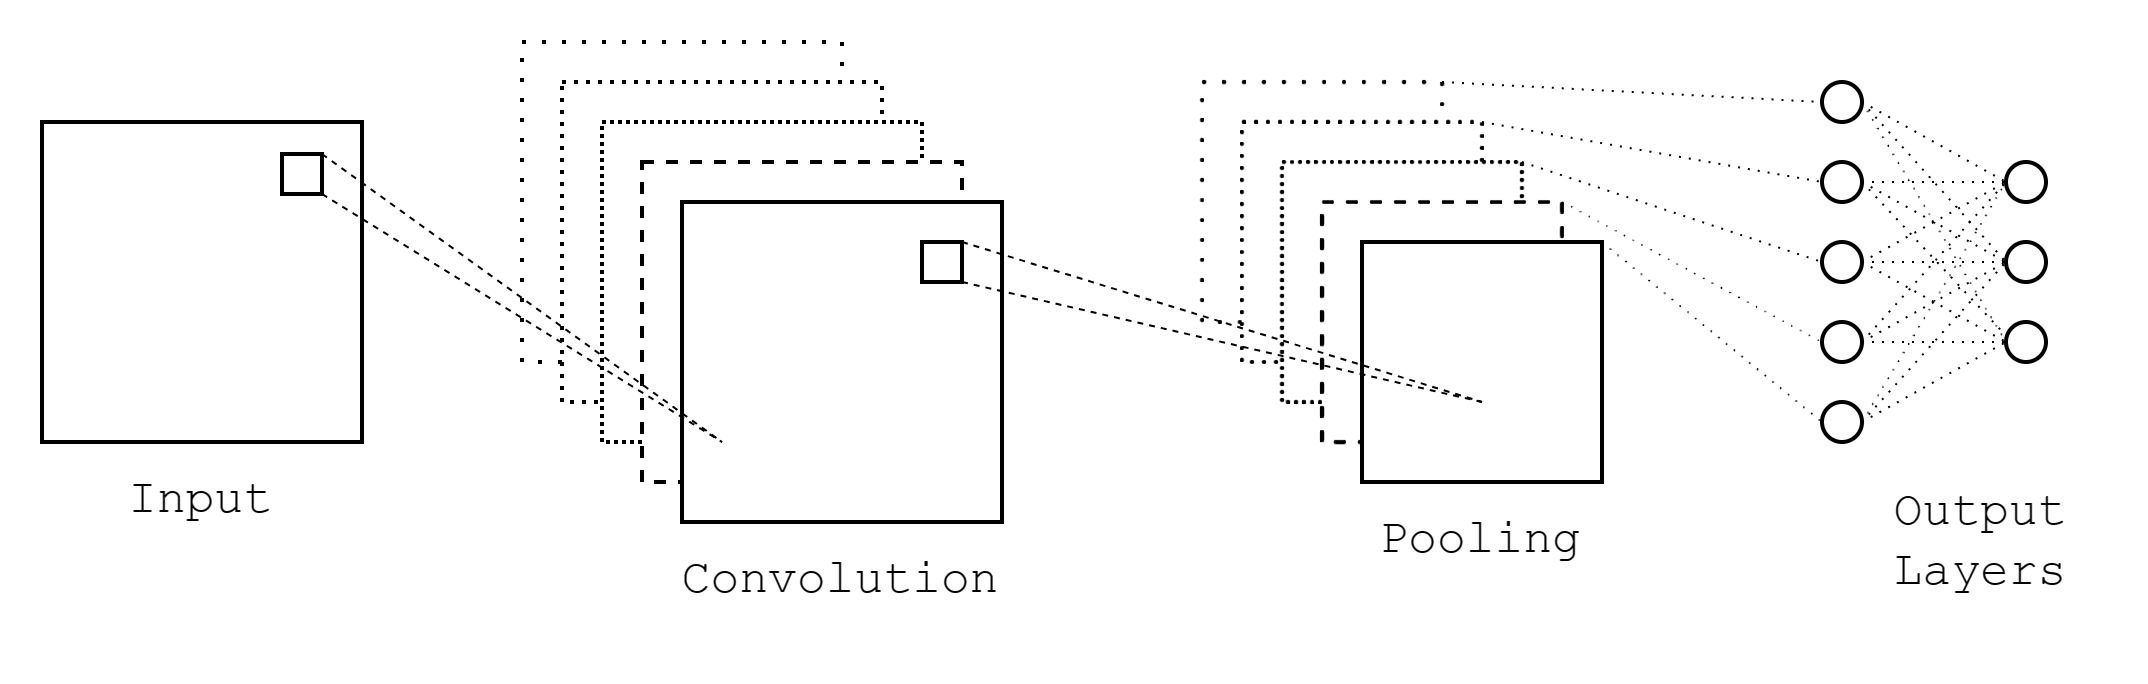
\includegraphics[width = \linewidth]{2}}
\caption{Pictorial representation of the CNN Architechture. There are 3 layers in a standard CNN Model - Convolution Layer, the central component of a CNN in which the bulk of computation takes place. It needs Input data, a kernal, and a feature map, among other things. The first convolution layer may be followed by another. When this occurs, the CNN's structure may become hierarchical because the later layers will be able to view the pixels in the earlier layers' receptive fields. The second layer being Pooling Layer, carries out dimensionality reduction, minimising the number of input parameters. Finally, we have Fully Connected output Layer, carries out the classification operation using the characteristics that were retrieved from the preceding layers and their various filters. Fully connected layers often utilise a \textit{Softmax Activation Function} [17] to categorise inputs adequately, producing a probability ranging from 0 to 1. Convolutional and pooling layers typically use \textit{ReLu functions.} [18]}
\end{figure}
\section{Dataset}
The dataset that is used to train the Convolutional Neural Network, is actually a subset of the \textit{Mars Reconnaissance Orbiter} dataset. We extracted the surface images of both, that had dunes, and devoid of any dunes. The modified dataset is made available publicly at \href{https://github.com/Anurag-Dutta/Prognosticate-Dunes-on-the-surface-of-Mars-using-Convolutional-Neural-Network/tree/main/dataset}{https://github.com/Anurag-Dutta/Prognosticate-Dunes-on-the-surface-of-Mars-using-Convolutional-Neural-Network/tree/main/dataset}. In both the training and testing data, the dataset was divided into 2 categories, those with dunes, and those without dunes. There were nearly, 1072 images corresponding to the first category, and 832 images corresponding to the second category. Figure 3 and 4 shows some instance of the data from both the categories. 
\begin{figure}[htbp]
\label{fig3}
\centerline{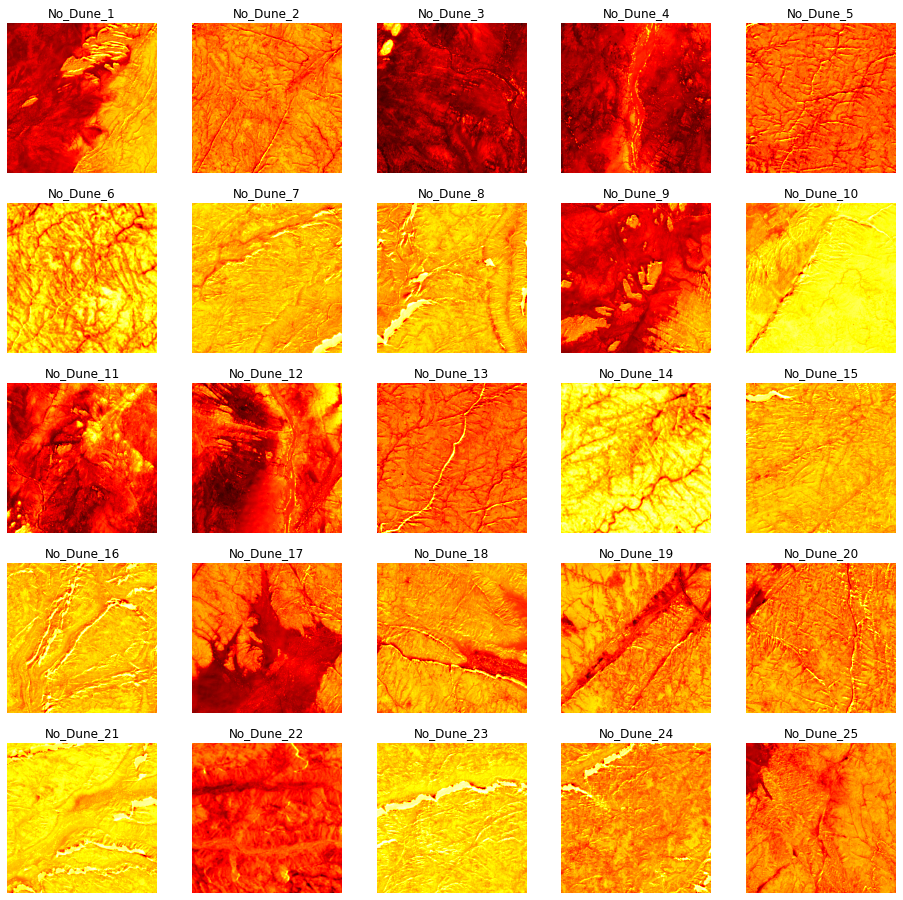
\includegraphics[width = \linewidth]{3}}
\caption{Martian Surficial Images without Dunes}
\end{figure}
\begin{figure}[htbp]
\label{fig4}
\centerline{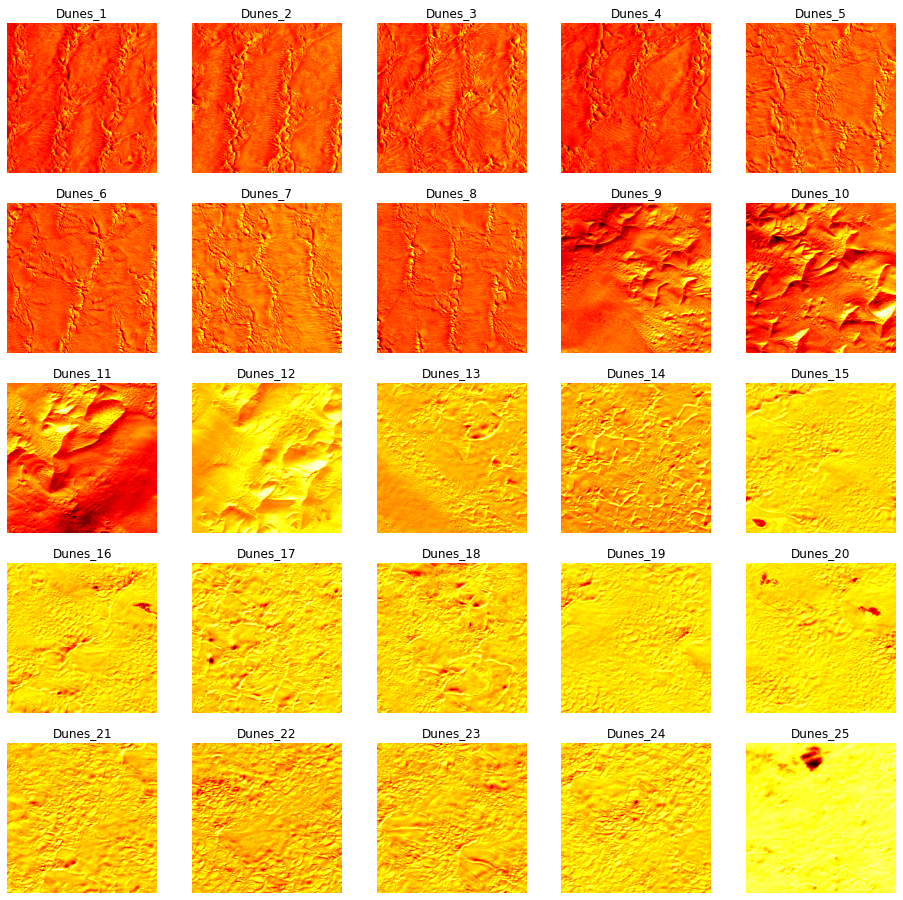
\includegraphics[width = \linewidth]{4}}
\caption{Martian Surficial Images with Dunes}
\end{figure}
\section{Results and Conclusion}
In this section, we would conclude the works of the article, by drawing out the results. Though, the primary model used for this work includes Convolutional Neural Network, we have also tried to converge the results making use of Traditional Classifiers, namely \textit{Gaussian Naive Bayes} [19], \textit{Random Forest} [20], \textit{k - Nearest Neighbours} [21], and a few more. While, the maximum accuracy that was potentially achieved by making use of these Classifiers, were nearly 80\%. Making, use of the \textit{Convolutional Neural Network}, we got a maximum accuracy of nearly 85\%. The results circumscribing the aforementioned paragraph have been shown below. 
\begin{verbatim}
==========================
[ Support Vector Machine ]
==========================

Training Accuracy = 0.7445830597504924
Testing Accuracy = 0.6771653543307087

\end{verbatim}
\begin{verbatim}
==========================
[ Random Decision Forest ]
==========================

Training Accuracy = 1.0
Testing Accuracy = 0.8320209973753281

\end{verbatim}
\begin{verbatim}
========================
[ Gaussian Naive Bayes ]
========================

Training Accuracy = 0.7078135259356533
Testing Accuracy = 0.6351706036745407

\end{verbatim}
\begin{verbatim}
=================
[ Decision Tree ]
=================

Training Accuracy = 1.0
Testing Accuracy = 0.6929133858267716

\end{verbatim}
\begin{verbatim}
==========================
[ k - Nearest Neighbours ]
==========================

Training Accuracy = 0.7931713722915299
Testing Accuracy = 0.7427821522309711

\end{verbatim}
Amonst all, the Random Forest Classifier worked with maximum accuracy. Figure 5 and 6 shows the Precision Recall Curve and Confusion Matrix of the Random Forest Classifier. 
\begin{figure}[htbp]
\label{fig5}
\centerline{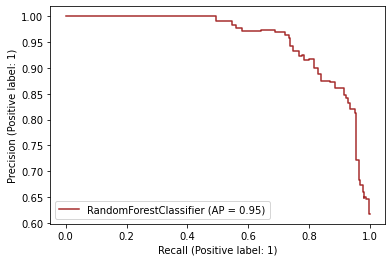
\includegraphics[width = \linewidth]{5}}
\caption{Precision Recall Curve of the Random Forest Classifier}
\end{figure}
\begin{figure}[htbp]
\label{fig6}
\centerline{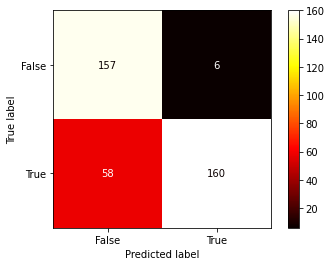
\includegraphics[width = \linewidth]{6}}
\caption{Confusion Matrix of the Random Forest Classifier}
\end{figure}
On the other hand, making use of the $\mathtt{sequential}$ CNN with 4 layers, $\mathtt{AdaGrad}$ optimizer, $\mathtt{binary\_crossentropy}$ as the loss function, and a total of 15 $\mathtt{epochs}$, the results were as, 
\begin{verbatim}
model.evaluate(validation_dataset)
\end{verbatim}
gave an output as follows, 
\begin{verbatim}
- loss: 0.4188 
- accuracy: 0.8211
[0.4187942147254944, 0.8211382031440735]
\end{verbatim}
Figure 7 and 8 shows the contrast of Validation with Training Accuracy, and the contrast of Validation with Training Loss.
\begin{figure}[htbp]
\label{fig7}
\centerline{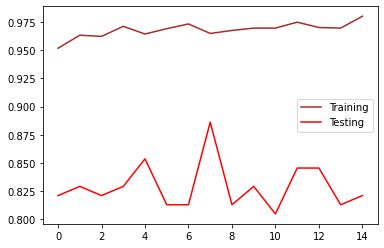
\includegraphics[width = \linewidth]{7}}
\caption{Plot contrasting Validation with Training Accuracy}
\end{figure}
\begin{figure}[htbp]
\label{fig8}
\centerline{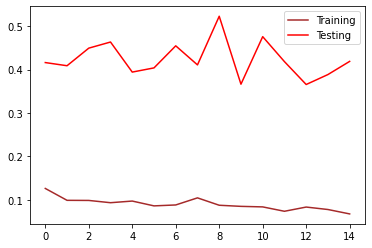
\includegraphics[width = \linewidth]{8}}
\caption{Plot contrasting Validation with Training Loss}
\end{figure}
\textbf{\\}

Even after using the Neural Network, we are getting a maximum accuracy of 85\%. We can make use of some advanced Neural Network, to get a better accuracy. Even, increasing the $\mathtt{epochs}$ to a considerable amount may cause a boost in the accuracy, or making use of some different optimizer would reduce the loss, and increase the accuracy. 
\begin{thebibliography}{00}
\bibitem{b1} J. Alves et al., “A Galactic-scale gas wave in the solar neighbourhood,” \textit{Nature}, vol. 578, no. 7794, pp. 237–239, Jan. 2020, doi: 10.1038/s41586-019-1874-z.
\bibitem{b2} R. Abuter et al., “A geometric distance measurement to the Galactic center black hole with 0.3\% uncertainty,” \textit{Astronomy \& Astrophysics}, vol. 625, p. L10, May 2019, doi: 10.1051/0004-6361/201935656.
\bibitem{b3} B. G. Bills, “Improved estimate of tidal dissipation within Mars from MOLA observations of the shadow of Phobos,” \textit{Journal of Geophysical Research}, vol. 110, no. E7, 2005, doi: 10.1029/2004je002376.
\bibitem{b4} A. Bagheri, A. Khan, M. Efroimsky, M. Kruglyakov, and D. Giardini, “Dynamical evidence for Phobos and Deimos as remnants of a disrupted common progenitor,” \textit{Nature Astronomy}, vol. 5, no. 6, pp. 539–543, Feb. 2021, doi: 10.1038/s41550-021-01306-2.
\bibitem{b5} P. K. Byrne, B. van Wyk de Vries, J. B. Murray, and V. R. Troll, “The geometry of volcano flank terraces on Mars,” \textit{Earth and Planetary Science Letters}, vol. 281, no. 1–2, pp. 1–13, Apr. 2009, doi: 10.1016/j.epsl.2009.01.043.
\bibitem{b6} T. A. Mutch et al., “The Surface of Mars: There View from the Viking 1 Lander,” \textit{Science}, vol. 193, no. 4255, pp. 791–801, Aug. 1976, doi: 10.1126/science.193.4255.791.
\bibitem{b7} “Scientific objectives and payloads of Tianwen-1, China’s first Mars exploration mission,” \textit{Advances in Space Research}, vol. 67, no. 2, pp. 812–823, Jan. 2021, doi: 10.1016/j.asr.2020.11.005.
\bibitem{b8} M. P. Golombek et al., “Overview of the Mars Pathfinder Mission and Assessment of Landing Site Predictions,” \textit{Science}, vol. 278, no. 5344, pp. 1743–1748, Dec. 1997, doi: 10.1126/science.278.5344.1743.
\bibitem{b9} A. H. Treiman, J. D. Gleason, and D. D. Bogard, “The SNC meteorites are from Mars,” \textit{Planetary and Space Science}, vol. 48, no. 12–14, pp. 1213–1230, Oct. 2000, doi: 10.1016/s0032-0633(00)00105-7.
\bibitem{b10} J. L. Vago et al., “Habitability on Early Mars and the Search for Biosignatures with the ExoMars Rover,” \textit{Astrobiology}, vol. 17, no. 6–7, pp. 471–510, Jul. 2017, doi: 10.1089/ast.2016.1533.
\bibitem{b11} T. J. Bayer, “In-Flight Anomalies and Lessons Learned from the Mars Reconnaissance Orbiter Mission,” \textit{2008 IEEE Aerospace Conference}, Mar. 2008, doi: 10.1109/aero.2008.4526483.
\bibitem{b12} D. T. Lyons, R. Stephen. Saunders, and D. G. Griffith, “The Magellan Venus mapping mission: Aerobraking operations,” \textit{Acta Astronautica}, vol. 35, no. 9–11, pp. 669–676, May 1995, doi: 10.1016/0094-5765(95)00032-u.
\bibitem{b13} J. P. Grotzinger, “Analysis of Surface Materials by the Curiosity Mars Rover,” \textit{Science}, vol. 341, no. 6153, pp. 1475–1475, Sep. 2013, doi: 10.1126/science.1244258.
\bibitem{b14} A. Yin, “Structural analysis of the Valles Marineris fault zone: Possible evidence for large-scale strike-slip faulting on Mars,” \textit{Lithosphere}, vol. 4, no. 4, pp. 286–330, Jun. 2012, doi: 10.1130/l192.1.
\bibitem{b15} K. FUKUSHIMA, “Neocognitron: Deep Convolutional Neural Network,” \textit{Journal of Japan Society for Fuzzy Theory and Intelligent Informatics}, vol. 27, no. 4, pp. 115–125, 2015, doi: 10.3156/jsoft.27.4\_115.
\bibitem{b16} L. Jiao et al., “A Survey of Deep Learning-Based Object Detection,” \textit{IEEE Access}, vol. 7, pp. 128837–128868, 2019, doi: 10.1109/access.2019.2939201.
\bibitem{b17} K. D. Onal et al., “Neural information retrieval: at the end of the early years,” \textit{Information Retrieval Journal}, vol. 21, no. 2–3, pp. 111–182, Nov. 2017, doi: 10.1007/s10791-017-9321-y.
\bibitem{b18} R. H. R. Hahnloser, R. Sarpeshkar, M. A. Mahowald, R. J. Douglas, and H. S. Seung, “Digital selection and analogue amplification coexist in a cortex-inspired silicon circuit,” \textit{Nature}, vol. 405, no. 6789, pp. 947–951, Jun. 2000, doi: 10.1038/35016072.
\bibitem{b19} D. J. Hand and K. Yu, “Idiot’s Bayes: Not So Stupid after All?,” \textit{International Statistical Review / Revue Internationale de Statistique}, vol. 69, no. 3, p. 385, Dec. 2001, doi: 10.2307/1403452.
\bibitem{b20} Tin Kam Ho, “The random subspace method for constructing decision forests,” \textit{IEEE Transactions on Pattern Analysis and Machine Intelligence}, vol. 20, no. 8, pp. 832–844, 1998, doi: 10.1109/34.709601.
\bibitem{b21} T. Cover and P. Hart, “Nearest neighbor pattern classification,” \textit{IEEE Transactions on Information Theory}, vol. 13, no. 1, pp. 21–27, Jan. 1967, doi: 10.1109/tit.1967.1053964.
\end{thebibliography}
\end{document}
